\documentclass[11pt,fancychapters]{report}
\usepackage[a4paper, total={6in, 8in}]{geometry}
\usepackage{listings}
\usepackage{color}
\usepackage{setspace}
\usepackage{hyperref}
\usepackage{acro}
\usepackage{amsmath}
\usepackage{amsthm}
\usepackage{amssymb}
\usepackage{amsfonts}
\usepackage{graphicx}
\usepackage{geometry}
\usepackage{cancel}
\usepackage{tikz}
\usepackage{subcaption}
\usepackage{bm}
\usetikzlibrary{calc,trees,positioning,arrows,chains,shapes.geometric,%
    decorations.pathreplacing,decorations.pathmorphing,shapes,%
    matrix,shapes.symbols}
\DeclareAcronym{etf}{
	short = ETF,
    long = Exchange-Traded Fund,
    class = abbrev
}

\DeclareAcronym{aum}{
	short = AUM,
    long = Assets Under Management,
    class = abbrev
}

\DeclareAcronym{sr}{
	short = SR,
    long = Sharpe Ratio,
    class = abbrev
}

\DeclareAcronym{nyse}{
	short = NYSE,
    long = New York Stock Exchange,
    class = abbrev
}

\DeclareAcronym{hft}{
	short = HFT,
    long = High Frequency Trading,
    class = abbrev
}

\DeclareAcronym{pv}{
	short = PV,
    long = present value,
    class = abbrev
}

\DeclareAcronym{fv}{
	short = FV,
    long = future value,
    class = abbrev
}

\DeclareAcronym{ir}{
	short = IR,
    long = interest rate,
    class = abbrev
}

\DeclareAcronym{capm}{
	short = CAPM,
    long = Capital Assets Pricing Model,
    class = abbrev
}

\DeclareAcronym{apt}{
	short = APT,
    long = Arbitrage Pricing Theory,
    class = abbrev
}

\DeclareAcronym{sma}{
	short = SMA,
    long = simple moving average,
    class = abbrev
}

\DeclareAcronym{mvo}{
	short = MVO,
    long = mean variance optimization,
    class = abbrev
}

\DeclareAcronym{rmse}{
	short = RMSE,
    long = root mean square error,
    class = abbrev
}

\DeclareAcronym{kNN}{
	short = kNN,
    long = k-nearest neighbor,
    class = abbrev
}
\geometry{top=1.3in,bottom=1.3in}
\hypersetup{
    colorlinks,
    citecolor=black,
    filecolor=black,
    linkcolor=black,
    urlcolor=black
}

\setcounter{secnumdepth}{4}

\definecolor{DarkerGreen}{RGB}{0,179,45}

\definecolor{Code}{rgb}{0,0,0}
\definecolor{Decorators}{rgb}{0.5,0.5,0.5}
\definecolor{Numbers}{rgb}{0.5,0,0}
\definecolor{MatchingBrackets}{rgb}{0.25,0.5,0.5}
\definecolor{Keywords}{rgb}{0,0,1}
\definecolor{self}{rgb}{0,0,0}
\definecolor{Strings}{rgb}{0,0.63,0}
\definecolor{Comments}{rgb}{0,0.63,1}
\definecolor{Backquotes}{rgb}{0,0,0}
\definecolor{Classname}{rgb}{0,0,0}
\definecolor{FunctionName}{rgb}{0,0,.7}
\definecolor{Operators}{rgb}{0,0,0}
\definecolor{Background}{rgb}{0.98,0.98,0.98}

\lstdefinestyle{python}{
  numbers=left,
  numberstyle=\footnotesize,
  numbersep=1em,
  xleftmargin=1em,
  framextopmargin=2em,
  framexbottommargin=2em,
  showspaces=false,
  showtabs=false,
  showstringspaces=false,
  frame=l,
  tabsize=4,
  % Basic
  basicstyle=\ttfamily\small\setstretch{1},
  backgroundcolor=\color{Background},
  language=Python,
  % Comments
  commentstyle=\color{Comments}\slshape,
  % Strings
  stringstyle=\color{Strings},
  morecomment=[s][\color{Strings}]{"""}{"""},
  morecomment=[s][\color{Strings}]{'''}{'''},
  % keywords
  morekeywords={import,from,class,def,for,while,if,is,in,elif,else,not,and,or,print,break,continue,return,True,False,None,access,as,,del,except,exec,finally,global,import,lambda,pass,print,raise,try,assert},
  keywordstyle={\color{Keywords}\bfseries},
  % additional keywords
  morekeywords={[2]@invariant},
  keywordstyle={[2]\color{Decorators}\slshape},
  emph={self},
  emphstyle={\color{self}\slshape},
  breaklines=true
}

\newtheorem{exmp}{Example}[section]

\newcommand{\codeExample}[2]{
	\begin{exmp}
      #1
      \noindent\begin{minipage}{\linewidth}
      \begin{lstlisting}[style=python]
          #2
      \end{lstlisting}
      \end{minipage}
    \end{exmp}
}

\newcommand\MyLBrace[2]{%
  \left.\rule{0pt}{#1}\right\}\text{#2}}
  
\tikzset{
>=stealth',
  punktchain/.style={
    rectangle, 
    rounded corners, 
    % fill=black!10,
    draw=black, very thick,
    text width=10em, 
    minimum height=3em, 
    text centered, 
    on chain},
  line/.style={draw, thick, <-},
  element/.style={
    tape,
    top color=white,
    bottom color=blue!50!black!60!,
    minimum width=8em,
    draw=blue!40!black!90, very thick,
    text width=10em, 
    minimum height=3.5em, 
    text centered, 
    on chain},
  every join/.style={->, thick,shorten >=1pt},
  decoration={brace},
  tuborg/.style={decorate},
  tubnode/.style={midway, right=2pt},
}

\title{Compiled Notes}
\author{Joseph Marino}

\begin{document}

\maketitle
\pagenumbering{gobble}
\newpage
\pagenumbering{roman}
\tableofcontents
\newpage
\pagenumbering{arabic}

\chapter{Intelligence}

\section{Intelligence}

Intelligence is a vaguely defined concept. In many situations, we often use the term to refer to the ability to perceive and understand certain concepts, such as math, art, politics, business, etc. But this narrow definition is human specific and fails to capture the broad spectrum that intelligence occupies. Instead, I use this working definition:

\begin{center}
	\textbf{Intelligence} is the ability of a system to perform meaningful actions within a particular environment.
\end{center}

We could argue whether a system that can perceive aspects of its environment but is unable to act is intelligent, but this is meaningless, as this system has no practical purpose. This definition has a few components: A \textbf{system} is some collection of matter: a molecular structure, single-celled organism, animal, machine, computer, human, society, etc. \textbf{Meaningful actions} are more difficult to define. In general terms, these are some non-random interactions with the environment, i.e. the distribution of actions given the environmental state has a relatively low entropy. Often we also associate these actions with achieving some goal or reward, although this is not strictly necessary. Finally, \textbf{within a particular environment} emphasizes the idea that intelligence is always specific to an environment (the data). Intelligence is not a characteristic of a system alone, it's always conditioned on the environment.

\section{Creating Intelligence}

There are two ways in which to create an intelligent system: through \textbf{design} and through \textbf{learning}. In design, one intelligent system constructs another intelligent system. In learning, a system gains intelligence through interaction with the environment.
\chapter{Probability \& Statistics}

Why define a system in terms of probability? Probability allows us to estimating uncertainty arising from stochasticity
\begin{itemize}
    \item in the system itself,
    \item in the measurement process, potentially the result of incomplete observability,
    \item due to limitations in the model, such as discretization.
\end{itemize}
There are two main interpretations of probability. The \textbf{frequentist} approach considers probabilities as the \textit{frequency} of events occurring, calculated over past trials. The \textbf{Bayesian} approach considers probabilities as a specifying the \textit{uncertainty} of events. Under the Bayesian interpretation, probability is a subjective belief, whereas under the frequentist interpretation, probability is an objective frequency of occurring events. While the basic rules of probability are consistent in both approaches, the advantage of the Bayesian approach is that it allows one to model uncertainty even when past trials have not necessarily been observed, providing flexibility. By expressing probability in terms of uncertainty, the Bayesian approach is also deeply connected to information theory (Chapter \ref{chap: information theory}), bringing additional mathematical tools for analysis. 

While probability gives us the tools to account for uncertainty in our estimates, it also brings a separate set of challenges associated with estimating various quantities. Rather than maintaining a single hypothesis about a quantity, probability often requires us to evaluate \textit{all} hypotheses. Instead of ``point estimates," we work with entire ``distributions." This creates computational difficulties stemming primarily from marginalization, i.e. summing or integrating over possible values. One common strategy for dealing with this is to forgo analytical estimates in favor of sampling-based estimates. In Chapter \ref{chap: variational inference}, we discuss variational inference, another technique for overcoming some of these issues.


\section{Probability}

Probabilities are defined for \textbf{random variables}, which can take either \textit{discrete} or \textit{continuous} values. A discrete variable could be whether or not a light switch is on, and a continuous variable could be the level of a light dimmer. A random variable only defines possible values that can be taken; to define the likelihood of the random variable taking each of the values, we must use a \textbf{probability distribution}. In the cases of the discrete and continuous random variables, the total probability of all values must sum to $1$ because the variable must take some value. The light switch must be on or off, and the light dimmer must be at some particular level. To accommodate this requirement, probabilities over discrete and continuous random variables must be handled differently, e.g. replacing summations with integrals, but the underlying rules of probability are identical in both cases.

\subsection{Discrete Random Variables}

Discrete random variables can take a finite or countably infinite number of values. Note that these values may not necessarily be numerical. In describing the probability over the values of a discrete random variable, we use a \textbf{probability mass function (PMF)}. A PMF, $P(x)$, is a function that maps discrete values of a random variable, $x$, to probabilities between $0$ and $1$, i.e.
$$\forall x, 0 \leq P(x) \leq 1. $$
Following our requirement that probability distributions must sum to $1$, we must ensure that
$$ \sum_x P(x) = 1. $$
We refer to a function meeting this requirement as being \textbf{normalized}. 

\subsection{Continuous Random Variables}

Continuous random variables take an uncountably infinite number of values, associated with a real value over some domain. To define the probability over this domain, we use a \textbf{probability density function (PDF)}. Unlike a PMF, a PDF, $p(x)$, is only required to be non-negative:
$$ \forall x, 0 \leq p(x). $$
Again, we must ensure that the total probability sums to $1$. Since we are dealing with a continuous domain, we must integrate:
$$ \int p(x) dx = 1. $$
Again, such a function is considered to be normalized. Note that $p(x)$ does not give the \textit{probability} of the value $x$, but rather, the probability \textit{density} at that point. In other words, with continuous random variables, we can only evaluate the probability of values in terms of intervals. In an infinitesimal interval, $\delta x$, around a point $x$, the probability is $p(x) \delta x$. More generally, we can quantify the probability mass within an interval $[a, b]$ as
$$P_{[a,b]} = \int_a^b p(x) dx. $$
In correspondence with physics, we can evaluate the probability \textit{mass} within an interval, i.e. \textit{volume}, by integrating the probability \textit{density} over that volume. This can also be accomplished by using the \textbf{cumulative density function (CDF)}, which is defined as
$$ \textrm{CDF}(x^\prime) \equiv \int_{- \infty}^{x^\prime} p(x) dx. $$
This allows us to quickly evaluate the probability within an interval as
$$ P_{[a,b]} = \textrm{CDF}(b) - \textrm{CDF}(a). $$

\subsection{Definitions and Rules}

The \textbf{joint distribution} defines the probability of events \textit{jointly} occurring over multiple variables. For instance, with variables $A$ and $B$, the joint distribution $p(A=a,B=b)$ defines the probability that variable $A$ takes the value $a$ \textit{and} variable $B$ takes the value $b$. The joint distribution can decomposed as
\begin{equation}
    p(A,B) = p(A|B)p(B) = p(B|A)p(A).
    \label{eq: def of joint prob}
\end{equation}
This decomposition is known as the \textbf{chain rule of probability}, and can be used to split any joint distribution into a series of \textbf{conditional} and \textbf{marginal distributions}. The conditional distribution defines the probability of an event in one variable occurring \textit{conditioned} on another event occurred in a different variable. Thus, $p(A=a | B=b)$ quantifies the probability that $A$ takes the value $a$ \textit{given} that $B$ takes the value $b$. Intuitively, this is defined as the probability of observing $a$ and $b$ together, divided by the probability of observing $b$ in general:
\begin{equation}
    p(A|B) = \frac{p(A,B)}{p(B)}.
    \label{eq: def of cond prob}
\end{equation}
The denominator here is the marginal distribution, which is obtained from the joint distribution over the variables by \textit{marginalizing}, i.e. summing, over the values of the other variables. To obtain the marginal $p(A)$, we marginalize over the variable $B$:
\begin{equation}
    p(A) = \sum_b p(A, B=b) = \sum_b p(A | B=b) p(B=b).
    \label{eq: def of marginal prob}
\end{equation}
From eq. \ref{eq: def of joint prob}, we can also jump directly to \textbf{Bayes' Rule}, which specifies one conditional probability, e.g. $p(A|B)$, in terms of the other conditional probability and the marginal distributions:
\begin{equation}
    p(A|B) = \frac{p(B|A)p(A)}{p(B)}.
    \label{eq: bayes rule}
\end{equation}

\section{Common Distributions}

\subsection{Probability Mass Functions}


\subsection{Probability Density Functions}


\subsection{Implicitly-Defined Distributions}

Up until now, we have discussed probability distributions that have a well-defined analytical form. These are sometimes referred to as \textit{explicitly-defined} distributions, because the form can be written down explicitly. However, there are also probability distributions that do not have an analytical form. These distributions are often defined in terms of invertible \cite{dinh2014nice} or non-invertible \cite{goodfellow2014generative} transformations of samples from other, simpler distributions. As the transformed distributions can only be evaluated through their samples, they are referred to as \textit{implicitly-defined} distributions \cite{mohamed2016learning}. In general, these distributions offer greater flexibility over explicitly-defined distributions, however, there are also additional difficulties associated with learning these distributions.
\chapter{Information Theory}

\section{Basic Concepts}

\textbf{Entropy} is a measure of the uncertainty of a random variable. It tends to agree with the notion of information. Let $X$ be a random variable, with alphabet $\mathcal{X}$ and probability mass function $p(x) = \text{Pr} (X = x)$, with $x \in \mathcal{X}$. The entropy of $X$ is defined as

\begin{equation}
	H(X) = - \sum_{x \in \mathcal{X}} p(x) \log p(x).
	\label{eq: entropy_definition}
\end{equation}

\noindent The units of entropy depend on the base of the logarithm. If the base is 2, then the units are in bits. If the base is $e$, then the units are in nats. To convert between different units of entropy, use $H_b (X) = (\log_b a) H_a (X)$. Note that entropy can be interpreted as the expectation of $-\log p(x)$. Also, entropy is non-negative: $H(X) \geq 0$.

The \textbf{joint entropy} of multiple random variables is defined similarly:

\begin{equation}
	H(X, Y) = - \sum_{x \in \mathcal{X}} \sum_{y \in \mathcal{Y}} p(x, y) \log p(x, y)
	\label{eq: joint_entropy_definition}
\end{equation}

\noindent Likewise, the \textbf{conditional entropy} is defined as

\begin{align*}
	H(Y | X) &= \sum_{x \in \mathcal{X}} p(x) H(Y | X = x) \\
		     &= - \sum_{x \in \mathcal{X}} p(x) \sum_{y \in \mathcal{Y}} p(y | x) \log p(y | x) \\
		     &= - \sum_{x \in \mathcal{X}} \sum_{y \in \mathcal{Y}} p(x, y) \log p(y | x).
	\label{eq: conditional_entropy_definition}
\end{align*}

\noindent Note that

\begin{equation}
	H(X, Y) = H(X) + H(Y | X).
\end{equation}

\noindent In words, joint entropy = individual entropy + conditional entropy. This also implies that

\begin{equation}
	H(X, Y | Z) = H(X | Z) + H(Y | X, Z).
\end{equation}

\noindent Because conditional entropy involves the conditional probability, we see that $H(Y | X) \neq H(X | Y)$. However,

\begin{equation}
	H(X) - H(X | Y) = H(Y) - H(Y | X).
\end{equation}

\textbf{Relative entropy} is a measure of the distance between two distributions. Put differently, it is the inefficiency of assuming the distribution of the data is $q(x)$ when the true distribution is $p(x)$. This is also referred to as the \textbf{Kullback-Leibler distance} or \textbf{divergence}.

\begin{equation}
	D_{KL} (p(x) || q(x)) = \sum_{x \in \mathcal{X}} p(x) \log \frac{p(x)}{q(x)} = \mathbb{E}_{x \sim p(x)} \Big[ \log \frac{p(x)}{q(x)} \Big]
	\label{eq: KL_definition}
\end{equation}

\noindent Note that if there is a value $x \in \mathcal{X}$ such that $p(x) > 0$ and $q(x) = 0$, then $D_{KL} = \infty$. KL divergence is non-negative and is only zero when $p(x) = q(x)$. It is not symmetric, so it is not a proper distance measure.

\textbf{Mutual Information} is the amount of information that one random variable contains about another random variable. In other words, it is the reduction in the uncertainty of one random variable due to knowledge of the other. It is expressed as the relative entropy between the joint distribution $p(x, y)$ and the product of the marginals $p(x) p(y)$.

\begin{align*}
	I(X; Y) &= \sum_{x \in \mathcal{X}} \sum_{y \in \mathcal{Y}} p(x, y) \log \frac{p(x, y)}{p(x) p(y)} \\
	           &= D_{KL} (p(x, y) || p(x) p(y)) \\
	           &= \mathbb{E}_{x, y \sim p(x, y)} \Big[ \log \frac{p(x, y}{p(x) p(y)} \Big].
\end{align*}

\noindent This can also be written as

\begin{equation}
	I(X; Y) = H(X) - H(X | Y) = H(Y) - H(Y | X).
\end{equation}

\noindent Thus, \textit{$X$ says as much about $Y$ as $Y$ says about $X$}. In words, mutual information is the amount of information in $X$ minus the amount of information in $X$ after observing $Y$ (and vice versa). This corresponds to the amount of information in $X$ that is explained by $Y$ (and, again, vice versa). If $Y$ perfectly explains $X$, then $H(X | Y) = 0$, so $I(X; Y) = H(X)$. At the other extreme, if $Y$ says nothing about $X$, then $H(X | Y) = H(X)$, so $I(X; Y) = 0$. Also, 

\begin{equation}
	I(X; Y) = H(X) + H(Y) - H(X, Y),
\end{equation}

\noindent and

\begin{equation}
	I(X; X) = H(X) - H(X | X) = H(X).
\end{equation}

\noindent Thus, entropy can be considered as the amount of self-information.

















\chapter{Neuroscience}

\section{Neurons}

\section{Neural Circuits}

\section{Brain Structures}
\chapter{Neural Networks}
\section{Basics}


\subsection{Linear Threshold Units}

\subsection{Multi-Layer Perceptrons}

\subsection{Backpropagation}


\chapter{Graphical Models}

\section{Latent Variable Models}

\subsection{Temporal Latent Variable Models}

We have a sequence of observations $\mathbf{x}_{\leq T}$, which extend over $T$ timesteps. Assume we also have a sequence of latent variables $\mathbf{z}_{\leq T}$. If we assume that time only moves in the forward direction, then with parameters $\theta$, we can write the joint probability of this model as

\begin{equation}
	p_\theta (\mathbf{x}_{\leq T}, \mathbf{z}_{\leq T}) = \prod_{t=1}^T p_\theta (\mathbf{x}_{t} | \mathbf{x}_{< t}, \mathbf{z}_{\leq t}) p_\theta (\mathbf{z}_{t} | \mathbf{x}_{< t}, \mathbf{z}_{< t}).
\end{equation}

\noindent The term $p_\theta (\mathbf{x}_{t} | \mathbf{x}_{< t}, \mathbf{z}_{\leq t})$ is the conditional likelihood or observation model, and the term $p_\theta (\mathbf{z}_{t} | \mathbf{x}_{< t}, \mathbf{z}_{< t})$ is the prior, transition, or dynamics model. The full graphical model is represented in figure \ref{fig: full_temporal_model}. The conditional dependencies show that the computation in this model grows exponentially with the sequence length $T$. Later, we will enforce stricter assumptions on the temporal dependencies to make computation tractable.

\begin{figure}[h]
    \centering
    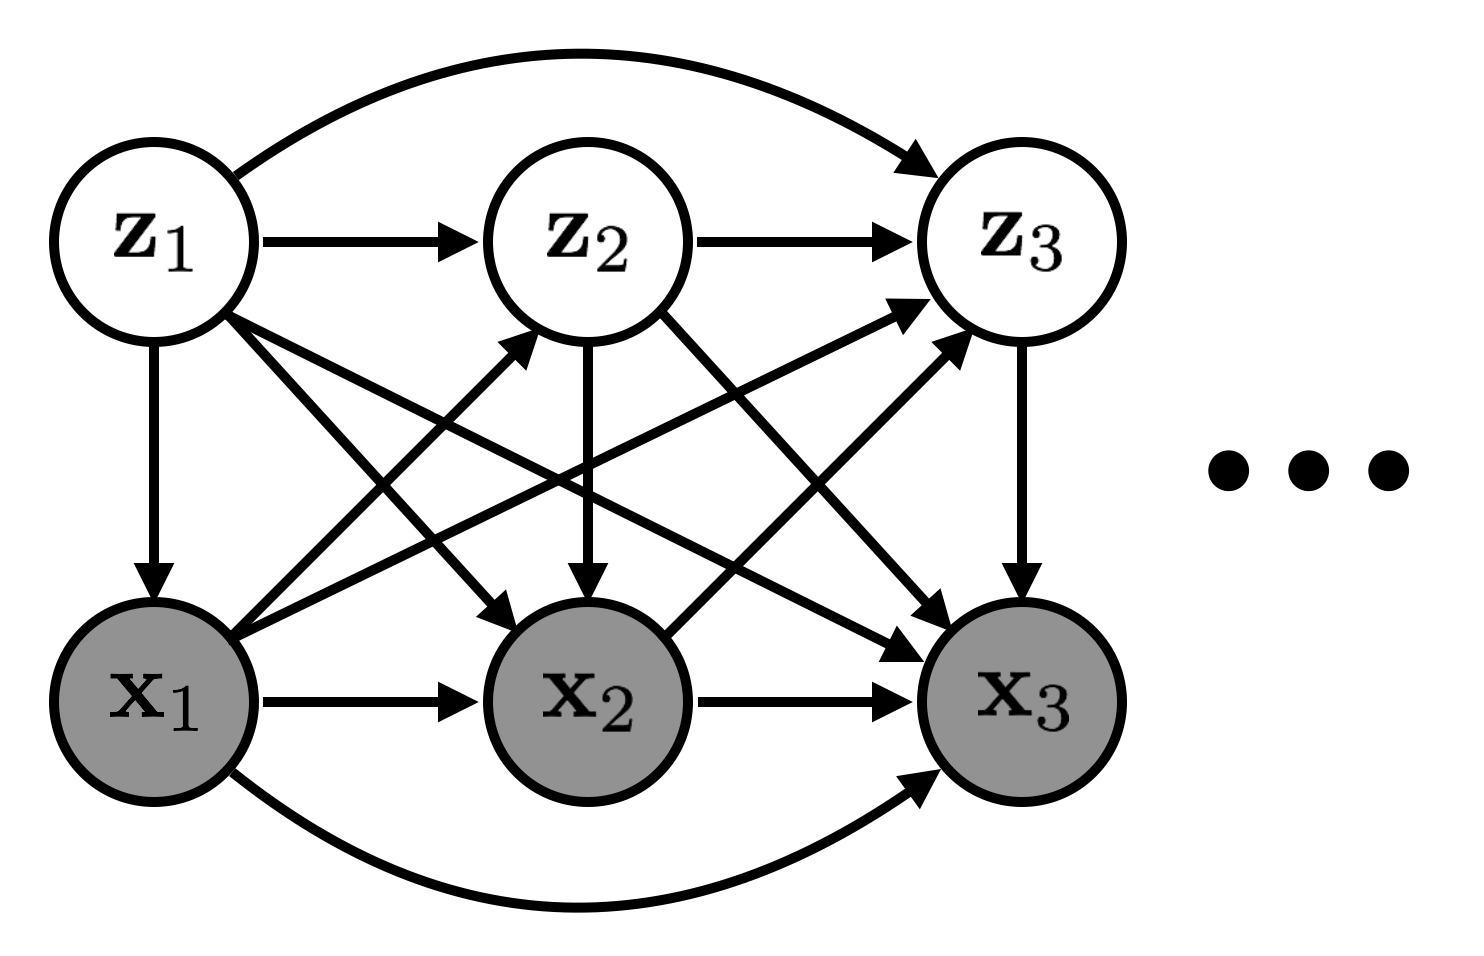
\includegraphics[width=.5\textwidth]{images/graphical_models/full_temporal_model.png}
    \caption{Simplified graphical model representation of temporal latent variable model with all connections present. Note that we're assuming the `arrow of time' points forward; variables can only affect other variables at the current time step or at future time steps. The parameters $\theta$ have been omitted for clarity.}
    \label{fig: full_temporal_model}
\end{figure}

To train or perform inference with this model, we need to compute $p_\theta (\mathbf{x}_{\leq T})$, which involves marginalizing over all states $\mathbf{z}_{\leq T}$:

\begin{equation}
	\log p_\theta (\mathbf{x}_{\leq T}) = \log \int p_\theta (\mathbf{x}_{\leq T}, \mathbf{z}_{\leq T}) d \mathbf{z}_{\leq T}
\end{equation}

\noindent Instead, we'll use an approximate posterior distribution, $q (\mathbf{z}_{\leq T} | \mathbf{x}_{\leq T})$, to compute a lower bound on this quantity:

\begin{equation}
	\log p_\theta (\mathbf{x}_{\leq T}) = \log \mathbb{E}_{q (\mathbf{z}_{\leq T} | \mathbf{x}_{\leq T})} \left[ \frac{p_\theta (\mathbf{x}_{\leq T}, \mathbf{z}_{\leq T})}{q (\mathbf{z}_{\leq T} | \mathbf{x}_{\leq T})} \right]
\end{equation}

\begin{equation}
	\log p_\theta (\mathbf{x}_{\leq T}) \geq \mathbb{E}_{q (\mathbf{z}_{\leq T} | \mathbf{x}_{\leq T})} \left[ p_\theta (\mathbf{x}_{\leq T}, \mathbf{z}_{\leq T}) - q (\mathbf{z}_{\leq T} | \mathbf{x}_{\leq T}) \right]
\end{equation}

\chapter{Variational Inference}
\label{chap: variational inference}

\section{Inference as Optimization: Deriving the ELBO}

Consider a model, $p(\mathbf{x}, \mathbf{z})$, that specifies a joint distribution over a latent variable $\mathbf{z}$ and observed variable $\mathbf{x}$. To infer the posterior distribution of $\mathbf{z}$ given $\mathbf{x}$, we can use the definition of conditional probability:

\begin{equation}
	p (\mathbf{z} | \mathbf{x}) = \frac{p(\mathbf{x}, \mathbf{z})}{p (\mathbf{x})},
	\label{eq: bayes rule}
\end{equation}

\noindent where the marginal likelihood (a.k.a. model evidence or partition function) $p(\mathbf{x})$ is calculated by marginalizing over the latent state space:

\begin{equation}
	p (\mathbf{x}) = \int p(\mathbf{x}, \mathbf{z}) d\mathbf{z}.
	\label{eq: marginalize}
\end{equation}

 \noindent For large latent spaces and/or complicated models, performing the integration in eq. \ref{eq: marginalize} is computationally intractable.
 
 Variational inference transforms this intractable integration problem into an \textit{optimization} problem by introducing an approximate posterior distribution, $q (\mathbf{z} | \mathbf{x})$, typically chosen from some simple family of distributions, such as independent Gaussians. We attempt to make $q (\mathbf{z} | \mathbf{x})$ as ``close" as possible to $p (\mathbf{z} | \mathbf{x})$ by minimizing $ D_{KL}(q (\mathbf{z} | \mathbf{x}) || p (\mathbf{z} | \mathbf{x}))$. Notice that the word close is in quotations because KL divergence is not a true distance measure; it is not symmetric. When the (non-negative) KL divergence between these distributions is zero, we recover the true posterior, $p (\mathbf{z} | \mathbf{x})$. We cannot evaluate $ D_{KL}(q (\mathbf{z} | \mathbf{x}) || p (\mathbf{z} | \mathbf{x}))$ directly, as it includes the true posterior, which we cannot tractably compute. Instead, we will maximize a lower bound on $p(\mathbf{x})$, which will have the effect of minimizing $ D_{KL}(q (\mathbf{z} | \mathbf{x}) || p (\mathbf{z} | \mathbf{x}))$, which we will now show. We start from the definition of KL divergence:
 
 \begin{equation}
 	D_{KL}(q (\mathbf{z} | \mathbf{x}) || p (\mathbf{z} | \mathbf{x})) = \mathbb{E}_{\mathbf{z} \sim q (\mathbf{z} | \mathbf{x})} \left[ \log \frac{q (\mathbf{z} | \mathbf{x})}{p (\mathbf{z} | \mathbf{x})} \right],
	\label{eq: elbo derivation 1}
 \end{equation}
 
 
 \begin{equation}
 	D_{KL}(q (\mathbf{z} | \mathbf{x}) || p (\mathbf{z} | \mathbf{x})) = \mathbb{E}_{\mathbf{z} \sim q (\mathbf{z} | \mathbf{x})} \left[ \log q (\mathbf{z} | \mathbf{x}) \right] - \mathbb{E}_{\mathbf{z} \sim q (\mathbf{z} | \mathbf{x})} \left[ \log p (\mathbf{z} | \mathbf{x}) \right].
	\label{eq: elbo derivation 2}
 \end{equation}
 
 \noindent Plugging in the definition of conditional probability into the second term yields:
 
  \begin{equation}
 	D_{KL}(q (\mathbf{z} | \mathbf{x}) || p (\mathbf{z} | \mathbf{x})) = \mathbb{E}_{\mathbf{z} \sim q (\mathbf{z} | \mathbf{x})} \left[ \log q (\mathbf{z} | \mathbf{x}) \right] - \mathbb{E}_{\mathbf{z} \sim q (\mathbf{z} | \mathbf{x})} \left[ \log \frac{p (\mathbf{x}, \mathbf{z})}{p (\mathbf{x})} \right],
	\label{eq: elbo derivation 3}
 \end{equation}
 
 \noindent which can be expanded into
 \begin{equation}
 	D_{KL}(q (\mathbf{z} | \mathbf{x}) || p (\mathbf{z} | \mathbf{x})) = \mathbb{E}_{\mathbf{z} \sim q (\mathbf{z} | \mathbf{x})} \left[ \log q (\mathbf{z} | \mathbf{x}) \right] - \mathbb{E}_{\mathbf{z} \sim q (\mathbf{z} | \mathbf{x})} \left[ \log p (\mathbf{x}, \mathbf{z}) \right] + \log p (\mathbf{x}).
	\label{eq: elbo derivation 4}
 \end{equation}
 
 \noindent Now, we'll define the following quantity, which we refer to as the \textit{evidence lower bound (ELBO)} or \textit{variational lower bound} or \textit{negative free energy}:
 
\begin{equation}
 	\boxed{\mathcal{L} \equiv \mathbb{E}_{\mathbf{z} \sim q (\mathbf{z} | \mathbf{x})} \left[ \log p (\mathbf{x}, \mathbf{z}) - \log q (\mathbf{z} | \mathbf{x}) \right]}
	\label{eq: elbo derivation 5}
\end{equation}

\noindent Plugging this definition back into eq. \ref{eq: elbo derivation 4}, we get

   \begin{equation}
 	D_{KL}(q (\mathbf{z} | \mathbf{x}) || p (\mathbf{z} | \mathbf{x})) = \log p (\mathbf{x})  - \mathcal{L}.
	\label{eq: elbo derivation 6}
 \end{equation}
 
 \noindent Rearranging terms, we see
 
    \begin{equation}
 	\log p (\mathbf{x})  =  \mathcal{L} + D_{KL}(q (\mathbf{z} | \mathbf{x}) || p (\mathbf{z} | \mathbf{x})).
	\label{eq: elbo derivation 7}
 \end{equation}

\noindent Since $D_{KL}(q (\mathbf{z} | \mathbf{x}) || p (\mathbf{z} | \mathbf{x}))$ is non-negative, $\mathcal{L}$ is a lower bound on $\log p (\mathbf{x})$. Further, since $\log p (\mathbf{x})$ is not dependent on $q (\mathbf{z} | \mathbf{x})$, we see that maximizing $\mathcal{L}$ with respect to $q (\mathbf{z} | \mathbf{x})$ must minimize $D_{KL}(q (\mathbf{z} | \mathbf{x}) || p (\mathbf{z} | \mathbf{x}))$. Thus, we can approximate the true posterior by optimizing $\mathcal{L}$ with respect to $q (\mathbf{z} | \mathbf{x})$.

Note that the ELBO can also be written in the following form:

\begin{equation}
 	\mathcal{L} = \mathbb{E}_{\mathbf{z} \sim q (\mathbf{z} | \mathbf{x})} \left[ \log p (\mathbf{x}, \mathbf{z}) - \log q (\mathbf{z} | \mathbf{x}) \right]
	\label{eq: elbo derivation 8}
 \end{equation}
 
\begin{equation}
 	\mathcal{L} = \mathbb{E}_{\mathbf{z} \sim q (\mathbf{z} | \mathbf{x})} \left[ \log p (\mathbf{x} | \mathbf{z})  + \log p(\mathbf{z}) - \log q (\mathbf{z} | \mathbf{x}) \right]
	\label{eq: elbo derivation 9}
 \end{equation}
 
\begin{equation}
 	\mathcal{L} = \mathbb{E}_{\mathbf{z} \sim q (\mathbf{z} | \mathbf{x})} \left[ \log p (\mathbf{x} | \mathbf{z}) \right] - D_{KL}(q (\mathbf{z} | \mathbf{x}) || p (\mathbf{z}))
	\label{eq: elbo derivation 10}
 \end{equation}

\noindent This highlights that the ELBO specifies the optimal $q (\mathbf{z} | \mathbf{x})$ by trading off between representing the input, through the first term, and agreeing with the prior on the latent variables, through the second term. In other words, the first term attempts to fit the data, while the second term regularizes the representation.



\section{Normalizing Flows} 

A common drawback of variational inference is that it is typically restricted to families of approximate posterior densities, e.g. factorized Gaussians. \textit{Normalizing flows} \cite{rezende2015variational} is a method for fitting flexible approximate posterior densities. It uses a sequence of invertible mappings, called a `flow,' to transform simple posterior densities into arbitrary, flexible forms. If we start with a variable $\mathbf{z}$, drawn from a distribution $q(\mathbf{z})$, and apply an invertible, smooth mapping $f(\mathbf{z})$, then the change of variables formula allows us to write

\begin{equation}
q(\mathbf{z}^\prime) = q(\mathbf{z}) \text{det} \bigg\vert \frac{\partial f^{-1}}{\partial \mathbf{z}^\prime} \bigg\vert = q(\mathbf{z}) \text{det} \bigg\vert \frac{\partial f}{\partial \mathbf{z}} \bigg\vert^{-1}.
\end{equation}
\newline

\begin{figure}[h]
    \centering
    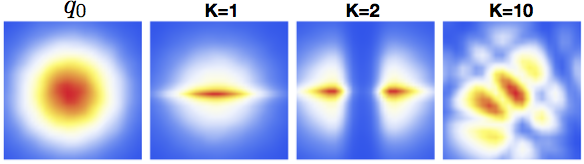
\includegraphics[width=.6\textwidth]{images/graphical_models/normalizing_flows.png}
    \caption{Normalizing flows applied to a 2D isotropic Gaussian, using transformations of the form given in eq. \ref{eq: normalizing flows transformation}. Increasing the flow length $K$ allows for more flexible approximate posterior distributions. Reproduced from \cite{rezende2015variational}.}
    \label{fig: normalizing flows}
\end{figure}

\noindent Note that the mapping, $f$, can also depend on other inputs, such as observed variables $\mathbf{x}$ or other auxiliary inputs. By composing multiple mappings, we can construct arbitrarily complex densities. Thus, starting from an initial distribution of $q_0 (\mathbf{z}_0)$, a flow of length $K$ can be computed as

\begin{equation}
	\log q_K (\mathbf{z}_K) = \log q_0 (\mathbf{z}_0) - \sum_{k=1}^K \log \text{det}  \bigg\vert \frac{\partial f_k}{\partial \mathbf{z}_{k-1}} \bigg\vert.
\end{equation}

\noindent This sequence can be interpreted as performing expansions and contractions on the initial density to construct a more flexible form. 

To parameterize the mappings, \cite{rezende2015variational} use transformations of the form

\begin{equation}
	f(\mathbf{z}) = \mathbf{z} + \mathbf{u}h(\mathbf{w}^\intercal \mathbf{z} + b)
	\label{eq: normalizing flows transformation}
\end{equation}

\noindent where $\mathbf{u}$, $\mathbf{w}$, and $b$ are learned parameters and $h(\cdot)$ is a non-linear function. This class of normalizing flows is referred to as $planar flows$. The determinant of the Jacobian of this transformation is

\begin{equation}
	\text{det} \bigg\vert  \frac{\partial f}{\partial \mathbf{z}} \bigg\vert = \big\vert \text{det} \left( \mathbf{I} + \mathbf{u} (h^\prime (\mathbf{w}^\intercal \mathbf{z} + b) \mathbf{w})^\intercal \right) \big\vert = \big\vert 1 + \mathbf{u}^\intercal h^\prime (\mathbf{w}^\intercal \mathbf{z} + b) \mathbf{w} \big\vert
\end{equation}

\noindent Finally, putting everything together, we can use normalizing flows to draw samples from the final, more flexible approximate posterior, $q(\mathbf{z} | \mathbf{x}) = q_K (\mathbf{z}_K)$. The variational lower bound becomes

\begin{equation}
	\mathcal{L} = \mathbb{E}_{\mathbf{z} \sim q(\mathbf{z}, \mathbf{x})} \left[ \log p(\mathbf{x}, \mathbf{z}) - \log q(\mathbf{z}|\mathbf{x}) \right]
	\label{eq: norm flows lower bound 1}
\end{equation}

\begin{equation}
	\mathcal{L} = \mathbb{E}_{\mathbf{z}_0 \sim q(\mathbf{z}_0, \mathbf{x})} \left[ \log p(\mathbf{x}, \mathbf{z}_K) - \log q(\mathbf{z}_0|\mathbf{x}) + \sum_{k=1}^K \log \big\vert 1 + \mathbf{u}_k^\intercal h_k^\prime (\mathbf{w}_k^\intercal \mathbf{z}_{k-1} + b_k) \mathbf{w}_k \big\vert \right]
	\label{eq: norm flows lower bound 2}
\end{equation}

\noindent Note that in going to eq. \ref{eq: norm flows lower bound 1} to eq. \ref{eq: norm flows lower bound 2} we have used the \textit{law of the unconscious statistician (LOTUS)}, which allows one to take expectations of a transformed variable (or any function thereof) using the original variable. If $\mathbf{z}^\prime = f(\mathbf{z})$ and $g$ is some arbitrary function of $\mathbf{z}^\prime$, then this can be expressed as

\begin{equation}
	\mathbb{E}_{\mathbf{z}^\prime \sim q (\mathbf{z}^\prime)} \left[ g(\mathbf{z}^\prime) \right] = \mathbb{E}_{\mathbf{z} \sim q (\mathbf{z})} \left[ g( f (\mathbf{z})) \right].
\end{equation}

\noindent Thus, we can take expectations with respect to the final density, i.e. the approximate posterior, using samples drawn from the initial density. In an amortized inference setting, the inference model can output the parameters of the initial distribution as well as parameters for each stage of the flow. The flow parameters could also be learned as global parameters.


Another class of normalizing flows is \textit{inverse auto-regressive flow (IAF)} \cite{kingma2016improved}. These transformations take inspiration from auto-regressive models, which factor joint probability distributions into a series of conditional distributions using the chain rule of probability.


\section{Filtering Variational Inference}
\label{sec: variational inference in dynamical models}

We assume the dynamic directed latent variable model set-up given in Section \ref{sec: dynamical latent variable models}. We can bound the marginal log-likelihood of the observation sequence by introducing an approximate posterior distribution, $q(\mathbf{z}_{1:T} | \mathbf{x}_{1:T})$, then using Jensen's inequality to write
\begin{equation}
    \log p(\mathbf{x}_{1:T}) \geq \mathbb{E}_{q(\mathbf{z}_{1:T} | \mathbf{x}_{1:T})} \left[ \log \frac{p(\mathbf{x}_{1:T} , \mathbf{z}_{1:T})}{q(\mathbf{z}_{1:T} | \mathbf{x}_{1:T})} \right] \equiv - \mathcal{F}_E,
    \label{eq: vi_1}
\end{equation}
where $\mathcal{F}_E$ is the total \textit{variational free-energy}. For now, we assume the generative model takes the form given by eq. \ref{eq: general dynamics model}, and the approximate posterior takes the form:
\begin{equation}
    q(\mathbf{z}_{1:T} | \mathbf{x}_{1:T}) = \prod_{t=1}^T q(\mathbf{z}_t | \mathbf{x}_{1:t} , \mathbf{z}_{1:t-1}).
    \label{eq: approx post form}
\end{equation}
In other words, we assume we are in the online setting, and therefore use a \textit{filtering} approximate posterior that does not condition on future observations or latent variables. Using eqs. \ref{eq: general dynamics model} and \ref{eq: approx post form}, we can rewrite eq. \ref{eq: vi_1} as
\begin{equation}
    \log p(\mathbf{x}_{1:T}) \geq \mathbb{E}_{q(\mathbf{z}_{1:T} | \mathbf{x}_{1:T})} \left[ \sum_{t=1}^T \log \frac{p(\mathbf{x}_t | \mathbf{x}_{1:t-1} , \mathbf{z}_{1:t}) p(\mathbf{z}_t | \mathbf{x}_{1:t-1} , \mathbf{z}_{1:t-1})}{q(\mathbf{z}_t | \mathbf{x}_{1:t} , \mathbf{z}_{1:t-1})} \right].
\end{equation}
Defining the term
\begin{equation}
    C_t \equiv \log \frac{p(\mathbf{x}_t | \mathbf{x}_{1:t-1} , \mathbf{z}_{1:t}) p(\mathbf{z}_t | \mathbf{x}_{1:t-1} , \mathbf{z}_{1:t-1})}{q(\mathbf{z}_t | \mathbf{x}_{1:t} , \mathbf{z}_{1:t-1})},
\end{equation}
then
\begin{align}
    \log p(\mathbf{x}_{1:T}) & \geq \mathbb{E}_{q(\mathbf{z}_{1:T} | \mathbf{x}_{1:T})} \left[ \sum_{t=1}^T C_t \right] \\
    & = \mathbb{E}_{q(\mathbf{z}_1 | \mathbf{x}_1)} \mathbb{E}_{q(\mathbf{z}_2 | \mathbf{x}_{1:2} , \mathbf{z}_1)} \dots \mathbb{E}_{q(\mathbf{z}_T | \mathbf{x}_{1:T} , \mathbf{z}_{1:T-1})} \left[ \sum_{t=1}^T C_t \right].
\end{align}
% \begin{align}
%     \log p(\mathbf{x}_{1:T}) & \geq \mathbb{E}_{q(\mathbf{z}_{1:T} | \mathbf{x}_{1:T})} \left[ \sum_{t=1}^T C_t \right] \\
%     & = \int_{\mathbf{z}_1} q(\mathbf{z}_1 | \mathbf{x}_1) \int_{\mathbf{z}_2} q(\mathbf{z}_2 | \mathbf{z}_1 , \mathbf{x}_{1:2}) \int_{\mathbf{z}_3} \dots \int_{\mathbf{z}_T} q(\mathbf{z}_T | \mathbf{z}_{1:T-1} , \mathbf{x}_{1:T}) \sum_{t=1}^T C_t
% \end{align}
There are $T$ terms within the sum, but because we do not condition on future variables, each $C_t$ only depends on the expectations up to time $t$. This allows us to write:
\begin{align}
    \log p(\mathbf{x}_{1:T}) & \geq \mathbb{E}_{q(\mathbf{z}_1 | \mathbf{x}_1)} \left[ C_1 \right] \nonumber \\ 
    & + \mathbb{E}_{q(\mathbf{z}_1 | \mathbf{x}_1)} \mathbb{E}_{q(\mathbf{z}_2 | \mathbf{z}_1 , \mathbf{x}_{1:2})} \left[ C_2 \right] \nonumber \\
    & + \dots \nonumber \\
    & + \mathbb{E}_{q(\mathbf{z}_1 | \mathbf{x}_1)} \mathbb{E}_{q(\mathbf{z}_2 | \mathbf{z}_1 , \mathbf{x}_{1:2})} \dots \mathbb{E}_{q(\mathbf{z}_T | \mathbf{z}_{1:T-1} , \mathbf{x}_{1:T})} \left[ C_T \right] \\
    & = \sum_{t=1}^T \mathbb{E}_{q(\mathbf{z}_{1:t} | \mathbf{x}_{1:t})} \left[ C_t \right] \\
    & = \sum_{t=1}^T \mathbb{E}_{\prod_{\tau=1}^t q(\mathbf{z}_\tau | \mathbf{x}_{1:\tau} , \mathbf{z}_{1:\tau-1})} \left[ C_t \right] \\
    & = \sum_{t=1}^T \mathbb{E}_{\prod_{\tau=1}^{t-1} q(\mathbf{z}_\tau | \mathbf{x}_{1:\tau} , \mathbf{z}_{1:\tau-1})} \left[ \mathbb{E}_{q(\mathbf{z}_t | \mathbf{x}_{1:t} , \mathbf{z}_{1:t-1})} \left[ C_t \right] \right]
\end{align}
% \begin{align}
%     \log p(\mathbf{x}_{1:T}) & \geq \int_{\mathbf{z}_1} q(\mathbf{z}_1 | \mathbf{x}_1) C_1 \\ 
%     & + \int_{\mathbf{z}_1} q(\mathbf{z}_1 | \mathbf{x}_1) \int_{\mathbf{z}_2} q(\mathbf{z}_2 | \mathbf{z}_1 , \mathbf{x}_{1:2}) C_2 \\
%     & + \dots \\
%     & + \int_{\mathbf{z}_1} q(\mathbf{z}_1 | \mathbf{x}_1) \int_{\mathbf{z}_2} q(\mathbf{z}_2 | \mathbf{z}_1 , \mathbf{x}_{1:2}) \dots \int_{\mathbf{z}_T} q(\mathbf{z}_T | \mathbf{z}_{1:T-1} , \mathbf{x}_{1:T}) C_T \\
%     & = \sum_{t=1}^T \mathbb{E}_{q(\mathbf{z}_{1:t} | \mathbf{x}_{1:t})} \left[ C_t \right] \\
%     & = \sum_{t=1}^T \mathbb{E}_{\prod_{\tau=1}^t q(\mathbf{z}_\tau | \mathbf{x}_{1:\tau} , \mathbf{z}_{1:\tau-1})} \left[ C_t \right] \\
%     & = \sum_{t=1}^T \mathbb{E}_{\prod_{\tau=1}^{t-1} q(\mathbf{z}_\tau | \mathbf{x}_{1:\tau} , \mathbf{z}_{1:\tau-1})} \left[ \mathbb{E}_{q(\mathbf{z}_t | \mathbf{x}_{1:t} , \mathbf{x}_{1:t})} \left[ C_t \right] \right] \\
% \end{align}
The total variational free-energy is thus the sum of per-time-step variational free-energies, with expectations taken w.r.t. all past latent variables:
\begin{equation}
    \mathcal{F}_E = - \sum_{t=1}^T \mathbb{E}_{\prod_{\tau=1}^{t-1} q(\mathbf{z}_\tau | \mathbf{x}_{1:\tau} , \mathbf{z}_{1:\tau-1})} \left[ \mathbb{E}_{q(\mathbf{z}_t | \mathbf{x}_{1:t} , \mathbf{z}_{1:t-1})} \left[ C_t \right] \right].
\end{equation}

Evaluating these outer expectations becomes computationally intractable as the sequence length grows. When approximating each of the $T$ expectations with $m$ Monte Carlo samples, evaluating the summation requires drawing $\mathcal{O}(m^T)$ samples. For $m > 1$, the number of samples, and therefore the amount of computation, blows up as $T \rightarrow \infty$. Thus, to retain tractability, we can set $m=1$ for expectations over all past time steps, thereby evaluating the path summation of the per time step variational free-energies, defined as the \textit{variational free-action}, $\mathcal{F}_A$:
\begin{equation}
    \mathcal{F}_A \equiv - \sum_{t=1}^T \mathbb{E}_{q(\mathbf{z}_t | \mathbf{x}_{1:t} , \mathbf{z}_{1:t-1})} \left[ C_t \right] \bigg \vert_{\mathbf{z}_{1:t-1}}
\end{equation}
where $\mathbf{z}_{1:t-1}$ is the sampled trajectory of the past latent variables. The free-action evaluates a single path through the latent space, whereas the free-energy evaluates all possible paths. However, the free-action still provides a lower bound on the marginal log-likelihood of the sequence. Need to show this...

\chapter{Representations \& Representation Learning}

\section{Motivation \& Definitions}

Overview of types of representations. How do we learning representations? What training criteria/conditions result in different representations? Are certain representations better than others? In which cases and why? The quality of a representation can only fundamentally be judged by its usefulness in helping to perform some task. That is, representations must be viewed in the context of a task.



\section{Disentangled Representations}

Define disentanglement. Why are disentangled representations helpful? Trade off between disentanglement and faithfully representing the data. How do we learn disentangled representations, while at the same time, respecting the structure of the latent space? Importance of priors.

Two random variables are \textbf{independent} if their joint probability can be expressed as the product of their marginals:

\begin{equation}
	p(\mathbf{x}, \mathbf{y}) = p(\mathbf{x}) p(\mathbf{y}),
\end{equation}

\noindent and they are \textbf{conditionally independent} if their conditional joint probability can be expressed as

\begin{equation}
	p(\mathbf{x}, \mathbf{y} | \mathbf{z}) = p(\mathbf{x} | \mathbf{z}) p(\mathbf{y} | \mathbf{z}).
\end{equation}

Independence is related to covariance, but is a stronger property. Two variables that are independent have zero covariance and two variables that have non-zero covariance are dependent. Zero covariance implies that the variables have no \textit{linear} dependence. Independence implies that the variables also have no \textit{non-linear} dependence. That is, it is possible for two dependent variables to have zero covariance. 
\\
\\
\noindent \textbf{Notes:}

\cite{cheung2014discovering} propose using a cross-covariance penalty term in the setting of semi-supervised learning of the form:

\begin{equation}
	C(\hat{\mathbf{y}}^{1 \dots N}, \mathbf{z}^{1 \dots N}) = \frac{1}{2} \sum_{ij} \left[ \frac{1}{N} \sum_n (\hat{y}^n_i - \bar{\hat{y}}_i) (z^n_j - \bar{z}_j) \right]^2,
\end{equation}

\noindent where $\hat{\mathbf{y}}$ is a vector of (one-hot) inferred labels and $\mathbf{z}$ is a latent representation. $N$ is the batch size.


\cite{higgins2016early} propose to use a regularization weight in a VAE setting to ``upweight" the amount of regularization as a means of promoting \textbf{redundancy reduction and independence} among the latent representation. They also argue for the importance of \textbf{dense sampling of the (continuous) data manifold} for disentanglement. Sparse sampling of the data manifold results in ambiguity is the manifold interpretation, requiring additional supervision for disentanglement.

\cite{siddharth2016inducing} use supervision to impose structure on part of the latent representation in a VAE.

Dropout \cite{srivastava2014dropout} is a technique for preventing ``fragile coadaptation" between units within a representation, effectively enforcing that they represent different (independent) quantities. This technique also results in redundancy within the representation.
\chapter{Reinforcement Learning}
\label{chap: reinforcement learning}

\section{The RL Problem Setting}

TODO: image of agent environment interaction.

\subsection{The Basics}

Reinforcement learning involves an \textbf{agent} interacting within an \textbf{environment}. The agent selects actions, and the environment responds with new states and rewards. Sutton \& Barto \cite{sutton1998reinforcement} identify four additional sub-elements to reinforcement learning systems:
\begin{itemize}
	\item a \textbf{policy},
	\item a \textbf{reward signal},
	\item a \textbf{value function},
	\item and, optionally, a \textbf{model} of the environment.
\end{itemize}
\noindent A \textit{policy} defines a mapping from (perceived) states to output actions to be taken. A \textit{reward signal} is a real-valued number that the agent receives from the environment. The agent tries to maximize its total reward, which is referred to as value. The \textit{value function} specifies the expected value, starting from a particular state. Thus, it is ultimately value that we try to optimize. Finally, a \textit{model} of the environment is the agent's simulation of the environment, allowing the agent to plan actions and predict outcomes (states, rewards, etc.).

The boundary between agent and environment is often not clearly defined. Sutton \& Barto place the agent-environment boundary at the limit of the agent's control, not at the physical boundary. For instance, the limbs of the agent, its internal energy reserves, and even the reward mechanism are considered to be part of the environment, since the agent does not have absolute control over these aspects.

We assume that time unfolds in a series of discrete time-steps, $t = 1, 2, 3, \dots$ At each time step, the agent is in some state $S_t \in \mathcal{S}$ and chooses some action $A_t \in \mathcal{A} (S_t)$. Here, $\mathcal{S}$ denotes the space of possible states and $\mathcal{A} (S_t)$ denotes the space of possible actions from state $S_t$. The action is chosen based on the agent's policy $\pi_t (a | s)$, which probabilistically maps states $S_t = s$ to actions $A_t = a$. At the next time step, the agent receives a real-valued reward, $R_{t+1} \in \mathcal{R} \subset \mathbb{R}$, and arrives in the next state, $S_{t+1}$.

The \textbf{return}, $G_t$, is the (discounted) sum of rewards starting at time $t$. For \textbf{episodic tasks}, in which the sequence has a finite length, $T$, this is defined as 

\begin{equation}
G_t \triangleq R_{t+1} + R_{t+2} + \dots + R_T = \sum_{k=0}^{T - t - 1} R_{t + k + 1},
\end{equation}

\noindent However, for \textbf{continuing tasks}, in which the time sequence length can be infinite, we include a \textbf{discount rate}, $\gamma \in [0, 1]$, to prevent the return from going to infinity:

\begin{equation}
G_t \triangleq R_{t+1} + \gamma R_{t+2} + \gamma^2 R_{t+3} + \dots = \sum_{k=0}^{\infty} \gamma^k R_{t + k + 1}.
\end{equation}

The \textbf{value function} or \textbf{state-value function}, $v_\pi (s)$, is defined as the expected return from being in state $s$ when using policy $\pi$:

\begin{equation}
	v_\pi (s) \triangleq \mathbb{E}_\pi \left[ G_t | S_t = s \right] = \mathbb{E}_\pi \left[ \sum_{k=0}^{\infty} \gamma^k R_{t + k + 1} | S_t = s \right].
	\label{eq: value_func_def}
\end{equation}

\noindent Note that here we are assuming that the task respects the Markov property; the current state, along with the policy, contains all of the information to determine the value function. We can also define an \textbf{action-value function}, $q_\pi (s, a)$, which specifies expected returns for each action $a$ taken from state $s$ using policy $\pi$:

\begin{equation}
	q_\pi (s, a) \triangleq \mathbb{E}_\pi \left[ G_t | S_t = s, A_t = a \right] = \mathbb{E}_\pi \left[ \sum_{k=0}^{\infty} \gamma^k R_{t + k + 1} | S_t = s, A_t = a \right].
\end{equation}

Using the definition of the value function, we can derive a recursive relationship known as the \textbf{Bellman equation}. Starting from eq. \ref{eq: value_func_def}:

\begin{align}
	\label{eq: bellman_0}
	v_\pi (s) &\triangleq \mathbb{E}_\pi \left[ G_t | S_t = s \right] \\
	\label{eq: bellman_1}
	&= \mathbb{E}_\pi \left[ \sum_{k=0}^{\infty} \gamma^k R_{t + k + 1} \bigg\vert S_t = s \right] \\
	\label{eq: bellman_2}
	&= \mathbb{E}_\pi \left[ R_{t+1} + \gamma \sum_{k=0}^{\infty} \gamma^k R_{t + k + 2} \bigg\vert S_t = s \right] \\
	\label{eq: bellman_3}
	&= \sum_{a, s^\prime, r} \pi(a | s) p(s^\prime, r | s, a) \left[ r + \gamma \mathbb{E}_\pi \left[ \sum_{k=0}^{\infty} \gamma^k R_{t + k + 2} \bigg\vert S_{t+1} = s^\prime \right] \right] \\
	\label{eq: bellman_4}
	&= \sum_{a, s^\prime, r} \pi(a | s) p(s^\prime, r | s, a) \left[ r + \gamma v_\pi (s^\prime) \right].
\end{align}

\noindent To go from eq. \ref{eq: bellman_1} to eq. \ref{eq: bellman_2}, we split the first term out of the sum. To arrive at \ref{eq: bellman_3}, we move the expectation to the future summation, re-expressing the expectation over the first step using summations to weight each return by the appropriate probability of the action $a$, state $s^\prime$, and reward $r$. Finally, to arrive at  \ref{eq: bellman_4}, we notice that the expectation is the value of state $s^\prime$ under our policy, i.e. $v_\pi (s^\prime)$. Thus, we see that the value function has the recursive definition:

\begin{equation}
	v_\pi (s) = \sum_{a, s^\prime, r} \pi(a | s) p(s^\prime, r | s, a) \left[ r + \gamma v_\pi (s^\prime) \right].
\end{equation}

\noindent A similar recursive definition can be derived for $q_\pi (s, a)$.

The \textbf{optimal value function} $v_* (s)$

\subsection{Summary of Notation}


\section{Value Based Methods}

\subsection{Multi-Armed Bandits}

The multi-armed bandit problem is an example of a \textit{non-associative setting}, in which the agent only learns to act in one situation. This simplifies much of the reinforcement learning problem. In particular, the \textbf{multi-armed bandit} problem involves a situation with $k$ possible actions (sometimes referred to as arms, in analogy to slot machines), each with an associated value. The value of action $a$ is denoted as $q_* (a)$, the \textbf{action-value function}. The interaction between the agent and the environment consists of a series of episodes, each of duration 1 time step. At time step $t$, the agent takes \textbf{action} $A_t$ and receives \textbf{reward} $R_t$. Thus, for some action $A_t = a$, the action-value function is defined as

\begin{equation}
	q_* (a) \triangleq \mathbb{E} \left[ R_t | A_t = a \right].
\end{equation}

\noindent Note that rewards can be a stochastic function of the action chosen. $q_* (a)$ encodes the \textit{mean} reward of choosing action $a$. In multi-armed bandit problems, the action-value function is initially unknown. To optimize total reward, we must estimate the action-value function to find the action or actions with the highest reward. Selecting this action will then optimize reward. We refer to the \textbf{action-value estimates} at time step $t$ as $Q_t (a)$.

At any time step $t$, we can either \textbf{exploit} our current knowledge by choosing the action with the optimal action-value estimate, or we can \textbf{explore} other actions with non-optimal action-value estimates. Exploitation is a greedy process, which will likely yield higher rewards in the short-term. Exploration, on the other hand, may find better actions, which can later be exploited, allowing it to likely yield higher rewards in the long-term.

We can select actions according to different strategies. For instance, we could select the action with the optimal action-value estimate at each time step:

\begin{equation}
A_t = \text{argmax}_a Q_t (a)
\end{equation}

\noindent However, this policy will never explore other actions, and may therefore perform poorly in the long run. Another strategy is to select the action with the optimal action-value estimate with probability $1 - \epsilon$ and select a random action with probability $\epsilon$. This strategy is referred to as $\epsilon$\textbf{-greedy}.

\subsection{Dynamic Programming Methods}

\subsubsection{Policy Iteration}

\subsubsection{Value Iteration}

\subsection{Monte Carlo Methods}

\subsection{TD Learning}

\subsubsection{Q Learning}

\subsubsection{SARSA}



\section{Policy Search Methods}
\label{sec: policy search methods}

\subsection{REINFORCE}

\subsection{Actor-Critic Methods}


\section{Deep Reinforcement Learning}
\chapter{Predictive Coding}

\section{Introduction}

Predictive coding, in its current form, was formalized by \cite{rao1999predictive}. This theoretical neuroscience model posited that sensory processing is a filtering problem, in which latent states underlying the environmental stimuli are estimated according to their agreement with the observed input as well as prior beliefs about these quantities. This offered an explanation for ``extra-classical" receptive field effects in visual processing, in which stimuli outside the receptive field of a particular cortical neuron are able to affect that neuron's activity. This was explained as the result top-down prior beliefs.

However, the notion of perception as a generative process dates back to at least \cite{von1867handbuch}. \textit{TODO: mention other early work before Rao and Ballard with similar ideas}

Predictive coding claims that sensory processing, i.e. perception, is fundamentally about constructing a generative model of the input sensory signal. To perform \textit{inference} in this model (to perceive), the model uses its current estimate of the latent variables underlying the environment to generate reconstructions or predictions of the input. Using the residual (error) from this reconstruction or prediction, along with residuals from prior beliefs, the model updates its estimate of these latent variables. \textit{Learning} corresponds to updating the parameters of the generative model to improve these overall residuals.
\newline

\subsection{Literature Summary}

\noindent \cite{clark2013whatever} provides a survey of the area of predictive coding
\newline

\noindent \cite{friston2002functional, friston2003learning, friston2005theory} presents a free energy formulation of predictive coding that uses expectation maximization. Primarily focuses on the static setting. Puts forth a theory of cortical processing as carrying out predictive coding.
\newline

\noindent \cite{friston2003dynamic} presents \textit{dynamic causal modeling}.
\newline

\noindent \cite{friston2008variational} presents \textit{variational filtering}.
\newline

\noindent \cite{friston2008DEM} presents \textit{dynamic expectation maximization} (DEM).
\newline

\noindent \cite{friston2010generalised} presents \textit{generalized filtering}, which does not make the mean-field assumption and instead treats all unknown variables as conditionally dependent. This differs from variational filtering \cite{friston2008variational} in that it assumes the parameters and precisions also change with time, with a prior on smoothness of these changes.
\newline

\noindent \cite{feldman2010attention} claims that attention can be formulated as the adjustment of prior precisions in the predictive coding model.
\newline

\noindent \cite{friston2011action}, \cite{friston2013anatomy} , \cite{friston2015active} \cite{friston2016active_process}, \cite{friston2016active} discuss \textit{active inference}.
\newline

\section{The Static Setting}

\subsection{MAP State Estimation in a One--Level Model}

Consider a situation in which the value of a single latent variable $z$ must be inferred from a single observed variable $x$. This is represented by the graphical model in figure  \ref{fig: simple_latent_model}. Let $g$ denote a non-linear function defining how $z$ generates $x$. Assume that the generated output takes the form of a normal distribution with mean $\mu_x = g(z)$ and constant variance $\sigma^2_x$:

\begin{figure}
    \centering
    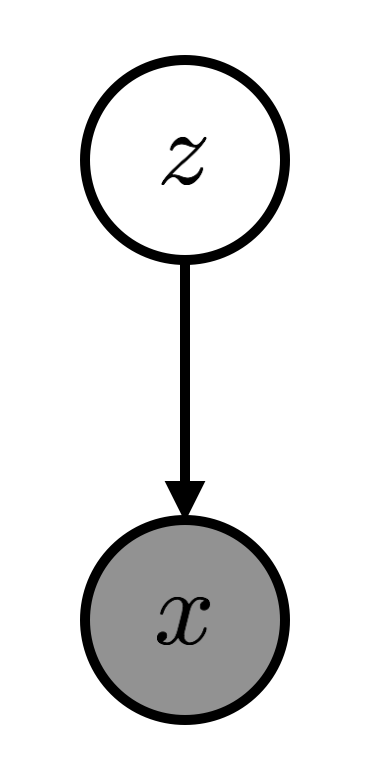
\includegraphics[width=0.15\textwidth]{images/predictive_coding/simple_latent_graphical_model.png}
    \caption{A graphical model denoting a latent variable model in which a single latent variable $z$ generates a single observed variable $x$. In predictive coding, we typically assume that $p(z)$ and $p(x|z)$ are Gaussian densities, and the generative mapping from $z$ to $x$ is a non-linear function.}
    \label{fig: simple_latent_model}
\end{figure}

\begin{equation}
	p (x | z) = \mathcal{N} (x; g(z), \sigma^2_x).
\end{equation}

\noindent Recall that in one dimension, a normal distribution takes the form

\begin{equation}
	\mathcal{N} (x; \mu, \sigma^2) = \frac{1}{\sqrt{2 \pi \sigma^2}} e^{-\frac{(x - \mu)^2}{2 \sigma^2}}.
	\label{eq: 1d gaussian}
\end{equation}

\noindent We will place a prior on $z$, which we also assume is a normal distribution with constant mean $\mu_p$ and constant variance $\sigma^2_p$:

\begin{equation}
	p (z) = \mathcal{N} (z; \mu_p, \sigma^2_p).
\end{equation}

\noindent To infer the posterior distribution of $z$, we can use Bayes' rule to invert the generative model:

\begin{equation}
	p (z | x) = \frac{p(x | z) p(z)}{p(x)},
\end{equation}

\noindent where the marginal distribution in the denominator is given as

\begin{equation}
	p (x) = \int p(x | z) p(z) dz.
	\label{eq: intractable integration}
\end{equation}

In general, computing the exact posterior distribution is computationally intractable due to the integration over $z$ in eq. \ref{eq: intractable integration}. Instead, we'll resort to variational inference\footnote{We are not actually using variational inference here, since the maximum of $p(z | x)$ must also be the maximum of $p(x, z)$ through the definition of conditional probability: $p(z|x) = \frac{p(x, z)}{p(x)}$, since $p(x)$ does not depend on the value of $z$. } to find the maximum (mode) of the posterior, otherwise known as the maximum a posteriori or MAP estimate. This is the \textit{most likely} estimate of the value of $z$. We will define our approximate distribution, a point mass estimate at $\mu_q$, as $q(z|x) = \delta (z = \mu_q)$, with the MAP estimate denoted as $\hat{\mu}_q$.

We want to maximize the evidence lower bound (ELBO), $\mathcal{L}$:

\begin{equation}
	\mathcal{L} = \mathbb{E}_{z \sim q(z|x)} \left[ \log p(x, z) - \log q(z|x) \right] = \mathbb{E}_{z \sim q(z|x)} \left[ \log p(x|z) + \log p(z) - \log q(z|x) \right] 
	\label{eq: elbo 1}
\end{equation}

\begin{equation}
	\mathcal{L} = \log \left( \frac{1}{\sqrt{2 \pi \sigma_x^2}} e^{-\frac{(x - g(\mu_q))^2}{2 \sigma_x^2}} \right) + \log \left( \frac{1}{\sqrt{2 \pi \sigma_p^2}} e^{-\frac{(\mu_q - \mu_p)^2}{2 \sigma_p^2}} \right)
	\label{eq: elbo 2}
\end{equation}

\begin{equation}
	\mathcal{L} = -\frac{1}{2} \log ( 2 \pi \sigma_x^2 )  - \frac{(x - g(\mu_q))^2}{2 \sigma_x^2} - \frac{1}{2} \log ( 2 \pi \sigma_p^2 ) -\frac{(\mu_q - \mu_p)^2}{2 \sigma_p^2}
	\label{eq: elbo 3}
\end{equation}

\begin{equation}
	\mathcal{L} = \frac{1}{2} \left( - \log ( \sigma_x^2 )  - \frac{(x - g(\mu_q))^2}{\sigma_x^2} - \log ( \sigma_p^2 ) -\frac{(\mu_q - \mu_p)^2}{\sigma_p^2} \right) + \text{const.}
	\label{eq: elbo 4}
\end{equation}

\noindent In going from eq. \ref{eq: elbo 1} to eq. \ref{eq: elbo 2}, we used the fact that $q(z|x)$ is a delta function, so the expectation becomes an evaluation at a single point, $z=\mu_q$. The expectation of $q(z|x)$ at this point is $1$, so $\log q(z|x)$ evaluates to $0$. To find the MAP estimate, we must solve the following optimization problem:

\begin{equation}
	\hat{\mu}_q = \text{argmax}_{\mu_q} \mathcal{L} =  \text{argmax}_{\mu_q} \frac{1}{2} \left( - \log ( \sigma_x^2 )  - \frac{(x - g(\mu_q))^2}{\sigma_x^2} - \log ( \sigma_p^2 ) -\frac{(\mu_q - \mu_p)^2}{\sigma_p^2} \right).
\end{equation}

\noindent To use first-order optimization methods, we must find the partial derivative of $\mathcal{L}$ w.r.t. $\mu_q$:

\begin{equation}
	\frac{\partial \mathcal{L}}{\partial \mu_q} = \frac{x - g(\mu_q)}{\sigma_x^2} \frac{d g}{d \mu_q} + \frac{\mu_q - \mu_p}{\sigma_p^2}
	\label{eq: 1d gradient}
\end{equation}

\noindent We see that we have two terms: \textbf{the first term moves the estimate toward agreement with the observation}, and \textbf{the second term moves the estimate toward agreement with the prior}. Each of these terms are weighted by their corresponding variances. In other words, inference (i.e. finding the optimal estimate of $\mu_q$) involves a weighted combination of \textit{bottom-up} and \textit{top-down} information. By repeatedly moving our estimate $\mu_q$ along this gradient, we can hopefully arrive at the MAP estimate $\hat{\mu}_q$. Note that we may not find the true value $\hat{\mu}_q$ if the optimization surface is non-convex. 

We would like to extend this single dimensional model to handle latent and observed variables of arbitrary size. In this setting, $\mathbf{x}$ and $\mathbf{z}$ are now vectors. The conditional likelihood, $p(\mathbf{x} | \mathbf{z}) = \mathcal{N} (\mathbf{x}; \bm{\mu}_\mathbf{x} = g(\mathbf{z}), \bm{\Sigma}_\mathbf{x})$ is now a multi-variate Gaussian distribution. The general form for this distribution is

 \begin{equation}
	\mathcal{N} (\mathbf{x}; \bm{\mu}, \bm{\Sigma}) = \frac{1}{(2 \pi)^{n/2} | \bm{\Sigma}|^{1/2}}  e^{-\frac{1}{2}(\mathbf{x} - \bm{\mu})^\intercal \bm{\Sigma}^{-1}(\mathbf{x} - \bm{\mu})},
	\label{eq: multi-variate gaussian}
\end{equation}

\noindent where $\bm{\Sigma}$ is the covariance matrix, $| \bm{\Sigma}|$ is the determinant of $\bm{\Sigma}$, and $n$ is the dimensionality of the vector $\mathbf{x}$. The prior on $\mathbf{z}$ is also a multi-variate Gaussian: $p(\mathbf{z}) = \mathcal{N} (\mathbf{z}; \bm{\mu}_p, \bm{\Sigma}_p)$. The MAP estimate is now a vector, $\hat{\bm{\mu}}_q$, of the most likely estimate of $\bm{\mu}_q$. To find this estimate, we must again optimize $\mathcal{L}$ w.r.t. $\bm{\mu}_q$. Repeating the steps above, the gradient, $\nabla_{\bm{\mu}_q} \mathcal{L}$, is given as:

\begin{equation}
	\nabla_{\bm{\mu}_q} \mathcal{L} =  \left( \frac{d g}{d \bm{\mu}_q} \right)^\intercal \bm{\Sigma}^{-1}_\mathbf{x} (\mathbf{x} - g(\bm{\mu}_q)) + \bm{\Sigma}^{-1}_p (\bm{\mu}_q - \bm{\mu}_p).
	\label{eq: multi-dimensional gradient}
\end{equation}

\section{The Dynamic Setting}

\section{Attention}

\section{Active Inference}

\section{Neural Implementation}

\subsection{Correspondence with Cortical Mircrocircuits}

\noindent \cite{bastos2012canonical} outlines ideas about correspondence between predictive coding and cortical microcircuits.
\newline

\noindent \cite{kanai2015cerebral} proposes that the pulvinar region of the thalamus is involved in setting precisions of predictions.
\newline

\noindent \cite{bogacz2017tutorial} gives an introductory tutorial to predictive coding with ideas about implementing predictive coding in neocortex.
\newline

\noindent \cite{whittington2017approximation} draws comparisons between backprop and predictive coding.
\newline


\chapter{Active Inference}
\label{chap: active inference}

The main idea behind Friston's more recent formulations of active inference is to explicitly set the model's prior over actions such that they minimize expected free energy (or maximize negative expected free energy). We have observations $\mathbf{x}$, hidden states $\mathbf{z}$, and control states $\mathbf{u}$, each of which are sequences. In Friston's formulations, these variables take discrete values. The generative model defines a joint distribution over these variables: $p (\mathbf{x}, \mathbf{z}, \mathbf{u})$. In \cite{friston2015active}, the model is factorized as:
\begin{equation}
    p (\mathbf{x}, \mathbf{z}, \mathbf{u}, \gamma | \mathbf{a}) = p(\mathbf{x} | \mathbf{z}) p(\mathbf{z} | \mathbf{a}) p(\mathbf{u} | \gamma) p(\gamma),
\end{equation}
\begin{equation}
    p(\mathbf{x} | \mathbf{z}) = p(\mathbf{x}_1 | \mathbf{z}_1) p(\mathbf{x}_2 | \mathbf{z}_2) \dots p(\mathbf{x}_t | \mathbf{z}_t),
\end{equation}
\begin{equation}
    p(\mathbf{z} | \mathbf{a}) = p(\mathbf{z}_2 | \mathbf{z}_1 , \mathbf{a}_1) p(\mathbf{z}_3 | \mathbf{z}_2 , \mathbf{a}_2) \dots p(\mathbf{z}_t | \mathbf{z}_{t-1} , \mathbf{a}_{t-1}),
\end{equation}
\begin{equation}
    p(\mathbf{u} | \gamma) = \sigma (\gamma \cdot \mathbf{Q} (\pi)),
\end{equation}
where $\mathbf{a}$ denotes past actions, $\sigma$ is the softmax function, and $\mathbf{Q} (\pi)$ is the negative expected free energy under policy $\pi$, which is defined as
\begin{equation}
    p(\mathbf{u} | \gamma) = \sigma (\gamma \cdot \mathbf{Q} (\pi)) = \sigma (\gamma \cdot \left[ \mathbf{Q}_{t+1} (\pi) + \mathbf{Q}_{t+2} (\pi) + \dots + \mathbf{Q}_T (\pi) \right] ),
\end{equation}
\begin{equation}
    \mathbf{Q}_\tau (\pi) \equiv \mathbb{E}_{q (\mathbf{x}_\tau , \mathbf{z}_\tau | \pi)} \left[ \log p(\mathbf{x}_\tau , \mathbf{z}_\tau | \pi) \right] + \mathbb{H} \left[ q (\mathbf{z}_\tau | \pi) \right].
\end{equation}
Here, $q (\mathbf{x}_\tau , \mathbf{z}_\tau | \pi)$ is the \textit{predictive posterior}, which is defined as
\begin{equation}
    q (\mathbf{x}_\tau , \mathbf{z}_\tau | \pi) = \mathbb{E}_{q(\mathbf{z}_\tau) } \left[ p (\mathbf{x}_\tau , \mathbf{z}_\tau | \mathbf{z}_t , \pi) \right].
\end{equation}
The expected free energy at time step $\tau$ can be written as
\begin{equation}
    \mathbf{Q}_\tau (\pi) \equiv \mathbb{E}_{q (\mathbf{x}_\tau , \mathbf{z}_\tau | \pi)} \left[ \log p(\mathbf{x}_\tau , \mathbf{z}_\tau | \pi) - \log q (\mathbf{z}_\tau | \pi) \right].
\end{equation}


\section{Introduction}

Active inference \cite{friston2009reinforcement} entails using action to reduce uncertainty or surprise. We have an agent within an environment. The agent maintains a generative model of the environment and itself, which is specified by the joint distribution $p_\theta (\mathbf{x}_{1:T}, \mathbf{z}_{1:T}, \mathbf{u}_{1:T})$, over sequences of observations $\mathbf{x}$, hidden states $\mathbf{z}$, and control states $\mathbf{u}$. Observations and states can be discrete, continuous, etc. A general form of the model is given by
\begin{equation}
    p_\theta (\mathbf{x}_{1:T}, \mathbf{z}_{1:T}, \mathbf{u}_{1:T}) = \prod_{t=1}^T 
\end{equation}


In active inference, the agent updates its (posterior) beliefs over hidden and control states to minimize surprise, the time average of $-\log p_\theta (\mathbf{x})$. As this is typically intractable to evaluate due to integration over hidden and control states, one can resort to minimizing an upper bound on surprise, the variational free energy, $\mathcal{F}$, using an approximate posterior distribution, $q (\mathbf{z}, \mathbf{u} | \mathbf{x})$:
\begin{equation}
    q^*(\mathbf{z}, \mathbf{u} | \mathbf{x}) = \argmin_q \mathcal{F}.
\end{equation}
The agent's control states (\textit{actions}) and hidden states (\textit{perceptions}) are then sampled from this approximate posterior distribution. The free energy can be written in a number of ways:
\begin{align}
    \mathcal{F} & = \mathbb{E}_{q (\mathbf{z}, \mathbf{u} | \mathbf{x})} \left[ -\log p_\theta (\mathbf{x}, \mathbf{z}, \mathbf{u}) + \log q (\mathbf{z}, \mathbf{u} | \mathbf{x}) \right] \\
    & =  D_{KL}(q (\mathbf{z}, \mathbf{u} | \mathbf{x}) || p_\theta (\mathbf{z}, \mathbf{u} | \mathbf{x})) - \log p_\theta (\mathbf{x}) \\
    & = \mathbb{E}_{q (\mathbf{z}, \mathbf{u} | \mathbf{x})} \left[ -\log p_\theta (\mathbf{x} | \mathbf{z}, \mathbf{u}) \right] + D_{KL}(q (\mathbf{z}, \mathbf{u} | \mathbf{x}) || p_\theta (\mathbf{z}, \mathbf{u}))
\end{align}
The first equation expresses free energy as Gibbs energy and entropy. The second equation shows that free energy upper bounds surprise, because KL divergence is non-negative. The third equation expresses free energy as a trade-off between model accuracy (first term) vs. model complexity (second term). \cite{friston2013anatomy} proposes a particular form for the generative model, in which the observation and latent dynamics models are factorized as follows:
\begin{equation}
    p_\theta (\mathbf{x}, \mathbf{z}, \mathbf{u}) = p_\theta (\mathbf{x} | \mathbf{z}) p_\theta (\mathbf{z}, \mathbf{u}),
\end{equation}
where the observation model is factorized across time as
\begin{equation}
    p_\theta (\mathbf{x} | \mathbf{z}) = \prod_{t=1}^T p_\theta (\mathbf{x}_t | \mathbf{z}_t),
\end{equation}
and the latent dynamics model is factorized across time as
\begin{equation}
    p_\theta (\mathbf{z}, \mathbf{u}) = p_\theta (\mathbf{u} | \mathbf{z}) \prod_{t=1}^T p_\theta (\mathbf{z}_t | \mathbf{z}_{t-1}, \mathbf{u}_{t-1})
\end{equation}
\begin{equation}
    \log p_\theta (\mathbf{u} | \mathbf{z}) = - \gamma \cdot D_{KL} (p_\theta (\mathbf{z}_{final} | \mathbf{z}, \mathbf{u}) || p_\theta (\mathbf{z}_{final}))
    \label{eq: distribution over actions}
\end{equation}
where $\mathbf{z}_{final}$ is the final hidden state. Goals are represented using the prior over final states, $p_\theta (\mathbf{z}_{final})$, expressing the preferences over which states the agent prefers to be in. By minimizing the control states, $\mathbf{u}$, the agent can attempt to bring itself toward its prior distribution over states, given it's current hidden state, $\mathbf{z}$. An advanced agent would be able to
\begin{itemize}
    \item set its own priors over states, potentially to highly abstract states that are not directly involved with physical rewards,
    \item optimize control states over long time horizons, making complex plans to achieve desired outcomes that are difficult to reach.
\end{itemize}
The specification of the distribution over actions (\ref{eq: distribution over actions}) can be decomposed as follows:
\begin{align}
    - D_{KL} (p_\theta (\mathbf{z}_{final} | \mathbf{z}, \mathbf{u}) || p_\theta (\mathbf{z}_{final})) & = \sum_{\mathbf{z}_{final}} p_\theta (\mathbf{z}_{final} | \mathbf{z}, \mathbf{u}) \log \frac{p_\theta (\mathbf{z}_{final})}{p_\theta (\mathbf{z}_{final} | \mathbf{z}, \mathbf{u})} \\
    & = H \left[ p_\theta (\mathbf{z}_{final} | \mathbf{z}, \mathbf{u}) \right] + \sum_{\mathbf{z}_{final}} p_\theta (\mathbf{z}_{final} | \mathbf{z}, \mathbf{u}) \log p_\theta (\mathbf{z}_{final})
\end{align}
The first term in this final expression is the entropy over final hidden states, which specifies the extent to which the agent has explored the states resulting from the environment. By treating $\log p_\theta (\mathbf{z}_{final})$ as the extrinsic reward or value of the corresponding state, the second term in the expression can be understood as the expected utility achieved by the agent for executing control states $\mathbf{u}$. This expression encompasses the exploration (first term) vs. exploitation (second term) trade-off. Note that if the prior over final states is uniform, i.e. the agent has no extrinsic rewards, then $\log p_\theta (\mathbf{z}_{final})$ is constant and can be brought outside of the sum. Because probability distributions sum to one, the exploitation term is a constant, and the agent simply takes actions for exploration. When the prior over states is non-uniform, this will bias the agent toward control states that are not purely exploratory, but are instead reward-seeking.

In more recent treatments, the formulation of active inference has been modified somewhat, where the KL divergence in eq. \ref{eq: distribution over actions} is replaced with the free energy. Thus, control states are selected to explicitly minimize free energy:
\begin{equation}
    \log p_\theta (\mathbf{u} | \mathbf{z}) = - \gamma \sum_t G_t (\mathbf{u})
\end{equation}
where $G_t (\mathbf{u})$ is the expected free energy for control states $\mathbf{u}$ at time $t$, defined as:
\begin{equation}
    G_t = \mathbb{E}_{q (\mathbf{z}, \mathbf{u} | \mathbf{x})} \left[  \right]
\end{equation}


\section{Literature Summary}

\noindent \cite{friston2011action}, \cite{friston2013anatomy} , \cite{friston2015active} \cite{friston2016active_process}, \cite{friston2016active} discuss active inference.

\chapter{Programming \& Experimental Practices}

This chapter contains some helpful practices for carrying out (machine learning) research projects.

\section{GitHub}

\href{https://github.com/}{GitHub} is an online platform for project source control. It is essential when collaborating on projects, as it allows you to meticulously track changes and manage conflicts between multiple versions of the code. But GitHub is also helpful when working alone on a project across multiple machines or if you just want to open source your code. The following are the basic commands for using GitHub:
\newline

\noindent \textbf{Clone a repository}:

\begin{lstlisting}[style=python]
git clone <repository address>
\end{lstlisting}

\noindent \textbf{Add a file to the repository}:

\begin{lstlisting}[style=python]
git add <filename>
\end{lstlisting}

\noindent \textbf{Or to add everything to the repository}:

\begin{lstlisting}[style=python]
git add .
\end{lstlisting}

or

\begin{lstlisting}[style=python]
git add -A
\end{lstlisting}

\noindent \textbf{Commit changes to the repository}:

\begin{lstlisting}[style=python]
git commit -m "<message>"
\end{lstlisting}

or

\begin{lstlisting}[style=python]
git commit
\end{lstlisting}

\noindent Note that if you run the second command, you will enter a vi interface where you can enter a multi-line message. To exit, type esc :wq

\noindent \textbf{Push all committed changes to the repository}:

\begin{lstlisting}[style=python]
git push
\end{lstlisting}

\noindent \textbf{Pull the repository}:

\begin{lstlisting}[style=python]
git pull
\end{lstlisting}

\noindent \textbf{To create a new branch}:

\begin{lstlisting}[style=python]
git branch <branch name>
\end{lstlisting}

\noindent \textbf{Switch current branch}:

\begin{lstlisting}[style=python]
git checkout <branch name>
\end{lstlisting}

\noindent \textbf{Merge branch changes back into master (while currently checking out other branch)}:

\begin{lstlisting}[style=python]
git merge master
\end{lstlisting}

\noindent You can send pull requests on GitHub.com. After the branch is merged, you can delete the branch on the website.
\newline

\noindent To conclude, a good workflow practice is to (1) pull the repository at the beginning of each work session, (2) push any incremental changes at regular intervals, and (3) create new branches for any major changes to be implemented.

\section{Logging}

Maintaining proper records of experiments is an essential part of conducting good research. Scientific notebooks (preferably in a digital format) are often helpful for keeping high-level notes about experiments, but one must keep experimental logs to track the different experimental set-ups that have been tested and the results. These are vital for surveying your project (what set-ups work? what set-ups should we consider trying?) and eventually communicating your results. Implementing and keeping track of these logs can seem like a hassle, but they are just as important as the experimental code itself.



\section{Plotting}


\bibliographystyle{ieeetr}
\bibliography{main}
\appendix
\chapter{Appendix 1} \label{App:AppendixA}

\end{document}